% IEEE Paper Template for US-LETTER Page Size (V1)
% Sample Conference Paper using IEEE LaTeX style file for US-LETTER pagesize.
% Copyright (C) 2006-2008 Causal Productions Pty Ltd.
% Permission is granted to distribute and revise this file provided that
% this header remains intact.
%
% REVISION HISTORY
% 20080211 changed some space characters in the title-author block
%
\documentclass[10pt,conference,letterpaper]{IEEEtran}
\usepackage{times,amsmath,epsfig}

%jing
\usepackage{graphicx}
\usepackage{balance}  % for  \balance command ON LAST PAGE  (only there!)
%
\usepackage{amsmath,amssymb}
%\usepackage[ruled]{algorithm2e}
\usepackage{xcolor}
\usepackage{caption2}
%\usepackage{verbatim}
\usepackage{url}
%%wj\usepackage{paralist}
%%wj\usepackage{lstautogobble}
%%wj\usepackage{listings}
%
%\usepackage{subcaption}
\usepackage{amsmath}
%\usepackage{bbold}
\usepackage{subfigure}
%\usepackage{enumitem}
\usepackage{textcomp}
%\usepackage{graphicx}
\usepackage{multirow}
\usepackage{comment}

%%wj
\begin{comment}
\lstset{%
	basicstyle=\ttfamily\small,
	identifierstyle=\rmfamily,
	keywordstyle=\rmfamily\bfseries,
	numbers=left,
	numberstyle=\footnotesize,
	numbersep=5pt,
	tabsize=3,
	frame=single,
	breaklines=true,
	breakatwhitespace=false,
	breakautoindent=true,
	mathescape=true,
	autogobble=true,
	linewidth=\linewidth,
	escapechar=@,
}
\end{comment}
%$wj

\usepackage{algorithm}
\usepackage{algpseudocode}
\usepackage{booktabs}

%%jing


%
%\title{\sys{}: Modeling the Retweeting Behaviors of User Groups in Social Media}
%\title{Grouping Users for Modeling Retweeting Behaviors}
\title{Incorporating User Grouping into \Retg{} Behavior Modeling}
% retweet or what?

%
\author{%
% author names are typeset in 11pt, which is the default size in the author block
{First Author{\small $~^{\#1}$}, Second Author{\small $~^{*2}$}, Third Author{\small $~^{\#3}$} }%
% add some space between author names and affils
\vspace{1.6mm}\\
\fontsize{10}{10}\selectfont\itshape
% 20080211 CAUSAL PRODUCTIONS
% separate superscript on following line from affiliation using narrow space
$^{\#}$\,First-Third Department, First-Third University\\
Address Including Country Name\\
\fontsize{9}{9}\selectfont\ttfamily\upshape
%
% 20080211 CAUSAL PRODUCTIONS
% in the following email addresses, separate the superscript from the email address 
% using a narrow space \,
% the reason is that Acrobat Reader has an option to auto-detect urls and email
% addresses, and make them 'hot'.  Without a narrow space, the superscript is included
% in the email address and corrupts it.
% Also, removed ~ from pre-superscript since it does not seem to serve any purpose
$^{1}$\,first.author@first-third.edu\\
$^{3}$\,third.author@first-third.edu%
% add some space between email and affil
\vspace{1.2mm}\\
\fontsize{10}{10}\selectfont\rmfamily\itshape
% 20080211 CAUSAL PRODUCTIONS
% separated superscript on following line from affiliation using narrow space \,
$^{*}$\,Second Company\\
Address Including Country Name\\
\fontsize{9}{9}\selectfont\ttfamily\upshape
% 20080211 CAUSAL PRODUCTIONS
% removed ~ from pre-superscript since it does not seem to serve any purpose
$^{2}$\,second.author@second.com
}
%



\begin{document}

%jing
\newtheorem{definition}{Definition}
\newtheorem{problem}{Problem}
\newtheorem{theorem}{Theorem}
\newtheorem{remark}{Remark}
\newtheorem{lemma}[theorem]{Lemma}
\newtheorem{corollary}[theorem]{Corollary}
%
\newcommand{\sys}{\textcolor{blue}{SYSNAME}}
\newcommand{\tbc}{\textcolor{blue}{[To Be Completed]}}
\newcommand{\retg}{\textcolor{blue}{retweeting}}
\newcommand{\retgs}{\textcolor{blue}{retweetings}}
\newcommand{\Retg}{\textcolor{blue}{Retweeting}}
\newcommand{\retd}{\textcolor{blue}{retweeted}}
\newcommand{\ret}{\textcolor{blue}{retweet}}
%%jing






\maketitle



\begin{abstract} 
Social media applications are emerging, with rapidly growing users and large numbers of \retd{} blogs every minute. 
The variety among users makes it difficult to model their \retg{} activities.
Obviously, it is not suitable to cover the overall users by a single model.
Meanwhile, building one model per user is not practical. 
To this end, this paper presents a novel solution, of which the principle is to model the \retg{} behavior over user groups.
Our approach, \sys{}, consists of three key components for extracting user based features, clustering users into groups, and modeling upon each group.
Particularly, we look into the user interest from different perspectives including long-term/recent interests and explicit/implicit interests, which results deep analyses towards the \retg{} behavior and proper models in the end.
We have evaluated the performance of \sys{} by datasets of real-world social networking applications and a number of query workloads, showcasing its benefits.     
\end{abstract}
% behavior and activity in this paper are interchangeable

\section{Introduction}
\label{sec:intro}

Social media is overwhelming nowadays, with massive users on Facebook, Twitter and Weibo while the number of users keeps increasing.
These users behave variously, knowledge of which is significant in recommendation system, activity prediction and Big Thing analysis.
Hence emerges the demand of developing systems and algorithms that could properly model user behaviors, which has already attracted the attention from both academia and industry.

Central to user behavior modeling, is the need to choose the granularity of model (i.e., how many users share one model), as well as the variety of features to be selected for differentiating these units.
Already, there exist work of building a single model for all the users \cite{IEEEexample:conf/wsdm/FengW13,IEEEexample:conf/ijcai/ZhangLTCL13,IEEEexample:journals/tkdd/ZhangTLLX15}.
Apparently, such model bears the limitation of being coarse.
On the other hand, modeling each user is not practical, due to the tremendous number of users.

The key driver of our work is the realization that in social media applications, users could fall into groups and each group shares representative behaviors.
%
As one example, consider the film \textit{Brave Heart}, fans of which are probably addicted to highland, bagpipe and war films, and thus likely to \ret{} blogs of these topics.
Particularly, we study the \retg{} behavior of users and our work can be generalized to other behaviors of like and comment as well. 
In the realm of social network behavior research, few work has been done towards making use of grouping, which however has been proved to be effective in other fields.
This motivates us to explore the incorporation of user grouping into the \retg{} behavior modeling, filling the gap of existed studies in literature.

\stitle{Contributions.}
This work contributes as follows:

\stab(1) We present a system named \sys{} with the novel perspective to model user behaviors over groups instead of the mono model in literature.

\stab(2) We leverage user interests to facilitate the modeling of \retg{} behavior and look into interests with various dimensions, including long-term/recent interests and explicit/implicit interests.

\stab(3) We evaluate the performance of \sys{} using real-world datasets, showcasing its benefits against competitive state of the art approaches.



\stitle{Organization.} The rest of this paper is organized as follows.
Section \ref{sec:overv} first gives the problem formulation and subsequently overviews \sys{}'s components, principle of which are detailed in Sections \ref{sec:fe}, \ref{sec:uc} and \ref{sec:gm} separately.
Section \ref{sec:perf} provides the performance evaluation.
Related work is presented in Section \ref{sec:rela}.
Finally, Section \ref{sec:conclu} concludes the work.












\section{Overview of System \sys{}}
\label{sec:overv}

%This section shall look into the principle of each component in Processing Runtime subsystem, putting forth a full-fledged system.

\subsection{Problem Formulation}
% {user, blog, user-blog} => model
% query (a user u, a blog b that is created or forwarded by u's friend)
% returns: Y/N u shall forward b

We consider people's \retg{} behavior in social media.
%For simplicity, with a given user, we assume that microblogs created or \retd{} by his/her followees cover the overall candidates, from which the said user may \ret{}.
For simplicity, assuming the microblogs that a user can \ret{} come from those owned by his/her followees.

%All our results could straightforwardly generalize to alternative candidate scopes.
%e.g., the like/unlike behavior against the candidate of remarking [double check the network language; register a Facebook]
%e.g., positive comments in the overall comments

\begin{definition}
\label{def:blog}
A microblog $M_b = (O, T, M, flag)$ has its owner $O$ (a.k.a. user in this paper) to whom $M_b$ belongs (either created or \retd{}), the generated time $T$ of $M_b$, the message context $M$, and $flag$ denoting $M_b$ is \retd{} (1) or originally created (0) by $O$.
\end{definition}

\begin{comment}
\begin{definition}
A blog $B = (O, T, M, C)$ consists of the owner $O$ to whom $B$ belongs (either created or \retd{}), the timestamp $T$ showing when $B$ is generated, the blog message $M$ and a set of counters $C_s(B) = \{\#comment,\ \#like,\ \#\ret{}\}$ regarding the number of being commented, liked, and \retd{}.
\end{definition}
\end{comment}

\begin{definition}
\label{def:user}
A user $u = (B_u, R_u, E_u)$ consists of three sets regarding the user's microblogs $B_u$, followers $R_u$ and followees $E_u$, in which each follower/followee per se refers to a user.
\end{definition}

%The mapping between blog $B$ and user $U$ is a bilateral operation, i.e., $U = O(B)$ and $B \in B_s(U)$, through ID(s) of user and blog respectively.
By Definition \textit{\ref{def:blog}} and \textit{\ref{def:user}}, $u = M_b.O$ and $M_b \in B_u$.
%
Providing a set of users $\mathbb{U}$ and the associated microblogs $\mathbb{B}$, as well as a microblog $b$ and a follower of $b.O$ written as $f$, i.e., $f \in R_{b.O}$, \sys{} builds a \retg{} model for $\mathbb{U}$ and $\mathbb{B}$, upon which 1/0 is returned regarding whether $f$ shall \ret{} $b$ or not.


\subsection{\sys{} Framework}
System \sys{} is designed from the ground up as a system for modeling users' \retg{} behavior in social media.
Figure \ref{fig:framework} shows the architectural components of \sys{}. %, mainly comprising Sina Microblog Data, Key Modules and Profile Demonstrator.

\begin{figure}[tb!]
\centering
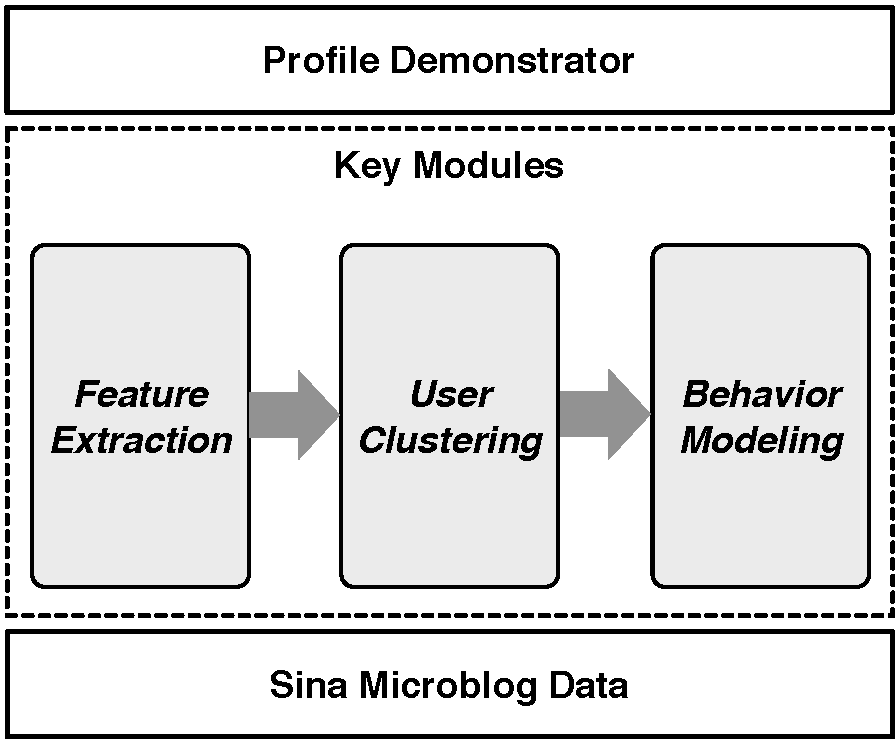
\includegraphics[width=.67\linewidth]{figures/architecture.pdf}
\vspace{-1ex}
\caption{\sys{} Architecture}
\label{fig:framework}
\vspace{-4ex}
\end{figure}


% #like and #comment are saved; could generalize \sys{} to model the liking behavior (among commented blogs)
\begin{comment}
\begin{figure}[!htb]
\centering
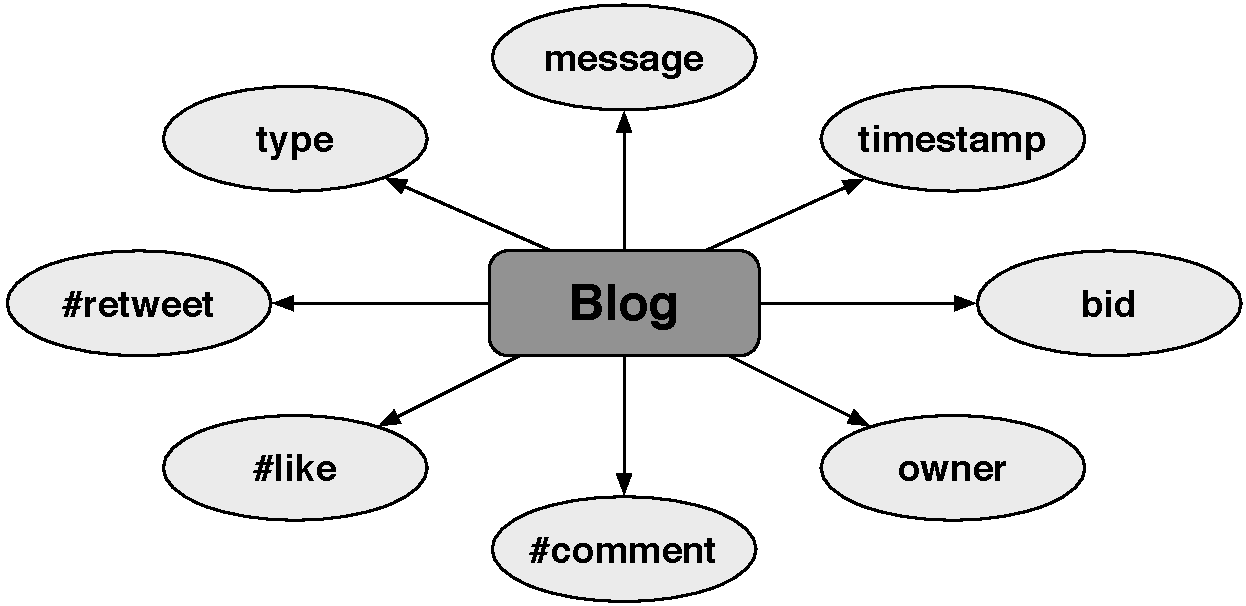
\includegraphics[width=.99\linewidth]{figures/microblog}
\caption{Blog Data in \sys{}}
\label{fig:blog}
\end{figure}
\end{comment}

\begin{comment}
\begin{figure}[!htb]
\centering
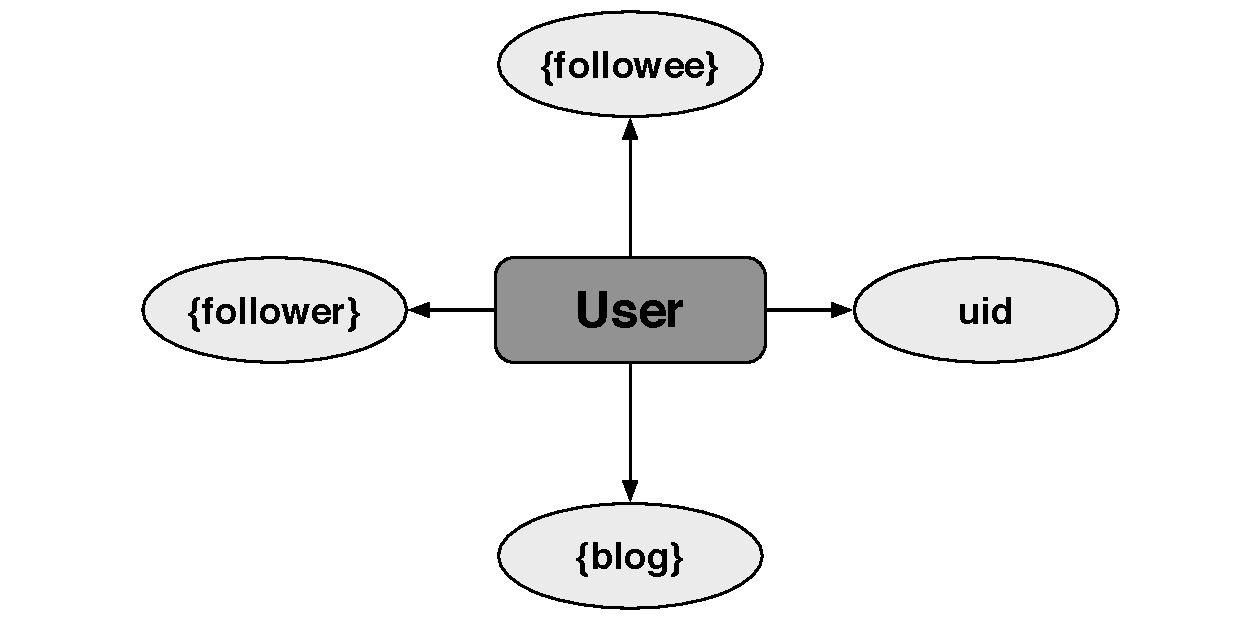
\includegraphics[width=.99\linewidth]{figures/user}
\caption{User Data in \sys{}}
\label{fig:user}
\end{figure}
\end{comment}


\stitle{Sina Microblog Data.} It is the data to be processed by \sys{}, i.e., data of microblogs and users, as shown in \textit{Definitions} \textit{\ref{def:blog}} and \textit{\ref{def:user}}.

\stitle{Key Modules.}
\sys{} consists of three key modules.
%\begin{enumerate}

	\stab(1)  Feature Extraction: By coalescing the microblog data, each user is depicted by a bunch of features, which are grouped into three categories. They are features of \textit{Basics} (e.g., the number of followers and followees), \textit{Behavior} (e.g., the frequency and the popular slots of \retg{}) and \textit{Interest} (e.g., the long-term/recent interests, as well as the explicit/implicit interests). These features are extracted from the stored  Sina Weibo data by Feature Extraction module, and serve as the input of the User Clustering module.
	
	\stab(2)  User Clustering: Providing the user-based features, User Clustering takes charge of the clustering task such that each user falls into a proper group.
	
	\stab(3)  Behavior Modeling: For each group obtained by User Clustering, Behavior Modeling builds a  model by employing both positive and negative samples (i.e., microblogs that are labeled with \retd{} and not \retd{}), over which the testing of users' \retg{} behavior is performed.
%\end{enumerate}
	
\stitle{Demonstrator.} At the top layer of \sys{}, it is the Demonstrator for visualizing all aspects of the system, e.g., profiling of user groups.
%For the time being, Profile Demonstrator presents \tbc{}.


As shown above, the distinctive feature of System  \sys{} is to model user \retg{} behaviors over groups instead of the mono model for all users.

\begin{table}[tb!]
\centering
\begin{small}
\caption{Illustration of Variables in Basic Feature}
\vspace{0.3cm}
\label{tbl:fe-info}
\begin{tabular}{ll}
\toprule
\multicolumn{1}{l}{\textbf{Variables}} & \multicolumn{1}{l}{\textbf{Illustration}}	\\	\midrule \midrule
\#$R_u$				& number of followers				\\	\midrule
\#$E_u$				& number of followees				\\	\midrule
                    & a ratio defined as the number of followers over \\
\raisebox{1.5ex}{$R_{ee}$}  & that of followees, i.e., ${\#R_u}/{\#E_u}$ \\  \midrule
$U_t$					& user type (as detailed in Table \ref{tbl:ucate})			\\ \bottomrule
\end{tabular}
\end{small}
\vspace{-3ex}
\end{table}
\begin{table}[tb!]
\centering
\begin{small}
\caption{Category of User Type}
\vspace{0.3cm}
\label{tbl:ucate}
\begin{tabular}{ll}
\toprule
\multicolumn{1}{l}{\textbf{Values}} & \multicolumn{1}{l}{\textbf{Illustration}}	\\	\midrule \midrule
0                       & $\#E_u \le 50 \ {\bf and} \ \#R_u \le 50$				\\	\midrule
\multirow{2}{*}{1}      & \multirow{2}{*}{$\frac{\#E_u}{\#R_u} \ \ge 5$}	\\
 						&                       									\\	\midrule
\multirow{2}{*}{2}		& \multirow{2}{*}{$\frac{\#R_u}{\#E_u} \ \ge 5$}  \\
						&															\\	\midrule
3                   	& other cases 												\\ \bottomrule
\end{tabular}
\end{small}
\end{table}



\section{\sys{} Principles}
\label{sec:prin}





\section{\sys{} Algorithms and Structures}
\label{sec:algo}
\section{Performance Evaluation}
\label{sec:perf}
\section{Related Work}
\label{sec:rela}
\section{Conclusions}

\label{sec:conclu}
\stitle{Acknowledgments}.
This work is supported in part by NSFC {\small U1636210}, 973 Program {\small 2014CB340300} \& NSFC {\small 61421003}. For any correspondence, please refer to Shuai Ma.








\cite{IEEEexample:article_typical}

\balance

\bibliographystyle{IEEEtran}
\bibliography{IEEEabrv,icde-zhu}

\end{document}
